% Conference derivative, condensed from overexpected.tex.
% Same claims ledger, same numbers, same figures. Prose is tightened, related
% work drops to a paragraph, practitioner implications gain weight.
\documentclass[10pt,letterpaper]{article}

\usepackage[T1]{fontenc}
\usepackage[utf8]{inputenc}
\usepackage{lmodern}
\usepackage[margin=0.9in]{geometry}
\usepackage{amsmath,amssymb}
\usepackage{booktabs}
\usepackage{graphicx}
\usepackage{caption}
\usepackage[round]{natbib}
\usepackage{microtype}
\usepackage[hidelinks]{hyperref}
\usepackage{siunitx}
\usepackage{titlesec}
\sisetup{detect-all, group-minimum-digits=4}

\titlespacing*{\section}{0pt}{1.4ex plus .2ex}{0.7ex}
\titlespacing*{\subsection}{0pt}{1.1ex plus .2ex}{0.5ex}
\captionsetup{font=small, labelfont=bf, skip=4pt}
\setlength{\parskip}{0pt}
\bibliographystyle{apalike}

\title{\vspace{-1.2cm}\bfseries Who Actually Draws Fouls?\\[2pt]
\large Measuring Foul-Drawing Skill from Public Play-by-Play,\\
and What a Leakage Audit Cost Us}

\author{Kevin Krajnc\\
\small Independent researcher \quad\textbar\quad \texttt{kevin@aandrs.at}\\
\small \url{https://github.com/quickstock/Over-Expected}}

\date{\vspace{-3mm}\small\today}

\begin{document}
\maketitle
\vspace{-6mm}

\begin{abstract}
\noindent\small
Free-throw attempts reward volume. A player who lives at the rim draws shooting
fouls whether or not he is good at drawing them. We model expected shooting-foul
free throws per possession from game context alone, never from shooter identity,
and define foul-drawing skill as the residual (FTAOE). The model runs on
\num{1420917} possessions across six NBA seasons, built entirely from public
play-by-play with no tracking data.

Two results matter for practitioners. First, a pre-publication audit found that
the public feed stamps score margin \emph{after} the event it describes, so a
margin feature in our companion expected field-goal model was encoding the shot's
own outcome. Fixing it moved holdout AUC from 0.6705 to 0.6578 and changed who
topped our published leaderboard. Anyone using this feed is exposed to the same
bug. Second, although the free-throw model improves on a season-mean baseline by
only \SI{0.195}{\percent} in Poisson deviance, the season-level metric is
reliable: split-half $r = 0.841$, full-season $r = 0.914$, year-over-year
$r = 0.85$ over \num{1691} qualified player-seasons, stabilising at
$K = 67$ possessions. Individual possessions are nearly unforecastable; players
are not. We also show that telling the model who is shooting raises
per-possession fit up to ninefold while barely moving the ordering, which is the
empirical case for keeping identity out.
\end{abstract}

\section{Why this metric}

``Who draws the most fouls'' is answered by usage and shot location before it is
answered by skill. Ranking players on free-throw attempts ranks them on role.
The quantity a front office actually wants is the residual: given the possessions
a player finished, did he draw more free throws than those possessions predicted?

We build that residual and call it FTAOE. A model predicts shooting-foul free
throws per possession from context that is external to the finisher: period,
game clock, the score margin the offence faced, home or away, the defending
team's foul rate, and the assigned officiating crew's foul rate. It never sees
who is shooting. FTAOE is actual minus predicted, anchored per season so the
league sums to zero and seasons stay comparable across rule-enforcement changes.

Everything runs on public NBA Stats play-by-play. No optical tracking is used,
which caps what the companion shot model can do and is stated plainly below. The
point of the exercise is that a useful player metric is reachable without a data
licence.

\paragraph{Related work.}
Shot quality is well covered publicly, from box-score decomposition
\citep{kubatko2007starting} to tracking-era possession value
\citep{cervone2016multiresolution}; foul drawing is not. The closest
neighbour is work separating where a player shoots from how well he converts
\citep{sandholtz2020measuring}, and the officiating literature establishing that
foul calls vary with referee and game state \citep{price2010racial}. We could not
find a public, reproducible expected-free-throw model reporting the reliability of
its player metric, so the figures below are given without a benchmark.

\section{Method}

\textbf{Data.} Six regular seasons, 2020--21 to 2025--26: \num{7230} games,
\num{1420917} possessions, \num{1282312} field-goal attempts. Possessions are
split with the \texttt{pbpstats} library rather than custom logic.

\textbf{Target.} \texttt{sfta} counts free throws awarded on a shooting foul,
including the and-one bonus shot. Technical, flagrant, clear-path,
away-from-play, inbound and penalty free throws are excluded, because they are
not caused by the act of shooting: \num{255738} free throws kept, \num{67569}
excluded, 533 contaminated trips dropped (\SI{0.085}{\percent}).

\textbf{Attribution.} Each possession is charged to a finisher: the free-throw
shooter, else the last player to score, else the player who turned it over, else
the last shooter. Every fouled possession has one; \SI{98.0}{\percent} of all
possessions do. Players qualify at 300 finisher-possessions, giving \num{1691}
qualified player-seasons.

\textbf{Model.} A Poisson GLM at possession grain on the seven context features
above. The opponent and crew rates are computed leave-one-game-out so a game
never enters its own predictor. Validation is a six-fold season cross-fit: train
on five seasons, predict the sixth, every prediction out-of-fold. Predictions are
then scaled per season to that season's observed league rate.

We tested two alternatives on identical folds. A multinomial logit over
$\{0,1,2,3^{+}\}$, which models the lumpy support directly, produced a
\emph{rank-identical} leaderboard ($\rho = 1.0000$). A Poisson LightGBM
\citep{ke2017lightgbm} improved per-possession fit to \SI{0.254}{\percent} but
moved full-season reliability only from 0.9135 to 0.9141, worsened calibration,
and again produced essentially the same ordering ($\rho = 0.9988$). We kept the
GLM.

\section{The leakage audit, and what it cost}

We audited the pipeline before publishing: target definitions, per-row
identities, feature timing, split construction, comparison to published league
aggregates, and direction checks. The important finding is a property of the data
source, not of our code.

\textbf{The score-margin field is stamped after the event it describes.} For a
made shot, it already contains that shot's points. Our expected field-goal model
used a feature derived from it, so the predictor partly encoded the outcome. We
verified the timing against the play-by-play sequence and retrained on an
identical split. Holdout AUC fell from 0.6705 to 0.6578, roughly 1.3 points of
apparent skill that was never real. Calibration barely moved (expected
calibration error 0.0040 to 0.0042), which is itself the tell: the leak inflated
ranking without distorting the probability scale, so a calibration check alone
would have missed it.

It changed published output. The 2024--25 leader in points over expected per 100
went from Jimmy Butler III (23.82) to Ty Jerome (22.99), with Butler at 22.42
once corrected.

Three further problems surfaced. xFG lacked season anchoring, so league-wide
points over expected per 100 drifted from $-1.70$ to $+1.07$ across seasons
instead of sitting near zero. Drawn free throws were valued at a hardcoded
\SI{77}{\percent} against actual league rates of \SI{77.5}{\percent} to
\SI{78.4}{\percent}. And a second margin leak in the free-throw model, once
fixed, moved no player-season by more than 1.03 free throws and changed no
season's top 20. Two leaks of the same class, very different consequences, and
only measurement told them apart. This is the practical lesson: find leaks by
auditing feature timing against the source, and size each one before deciding
whether it matters \citep{kaufman2012leakage}.

\section{Results}

\subsection{The fit statistic is not the useful number}

Out-of-fold Poisson deviance falls \SI{0.195}{\percent} against a season-mean
baseline. Read as a possession-level predictor, that is close to nothing, and we
are not going to dress it up.

Read as a measurement instrument it is fine. Splitting each qualified
player-season into odd and even games gives split-half $r = 0.841$, a
Spearman-Brown full-season figure of $r = 0.914$, and a padding constant of
$K = 67$ possessions. Year-over-year correlation averages 0.85 across five
consecutive-season pairs (0.852, 0.834, 0.859, 0.865, 0.840).

That combination is the finding. Whether a specific possession draws a shooting
foul is nearly unforecastable from public features. Whether a player draws them
at an unusual rate over a season is highly stable. Figure~\ref{fig:rel} shows
both, including how fast the metric stabilises.

\begin{figure}[t]
\centering
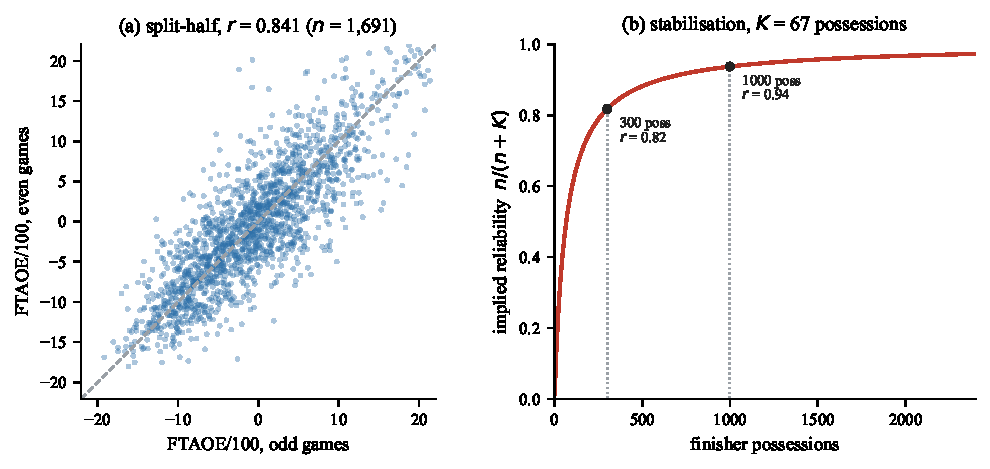
\includegraphics[width=\textwidth]{figures/fig2_ftaoe_reliability.pdf}
\caption{(a) Odd-game against even-game FTAOE per 100, \num{1691} qualified
player-seasons. (b) Implied reliability against sample size, $n/(n+K)$ with
$K = 67$ possessions.}
\label{fig:rel}
\end{figure}

\subsection{Telling the model who is shooting}

The model is context-only by design. To price that choice we refitted it twice on
identical folds, adding the finisher's height and position, then additionally his
prior-season free-throw rate.

Identity helps the fit a lot in relative terms: mean fold lift rises from
\SI{0.196}{\percent} to \SI{0.827}{\percent} to \SI{1.786}{\percent}. The
ordering barely cares. Rank correlation with the context-only board is
$\rho = 0.906$ and $\rho = 0.832$ respectively. The tail moves more than the
body, and we flag it rather than bury it: top-ten overlap is 6 of 10 and 2 of 10.

What the last arm really shows is circularity, and it is the clearest picture in
the paper. Prior-season free-throw rate measures the thing FTAOE measures. Supply
it and the model explains the signal away. Rudy Gobert's 2022--23 goes from
$+20.06$ to $-15.70$ per 100, the largest move in the sample, and he owns four of
the eight biggest drops (Figure~\ref{fig:identity}). Tell the model Gobert draws
fouls and he stops drawing them over expectation. That is why identity stays out.

\begin{figure}[t]
\centering
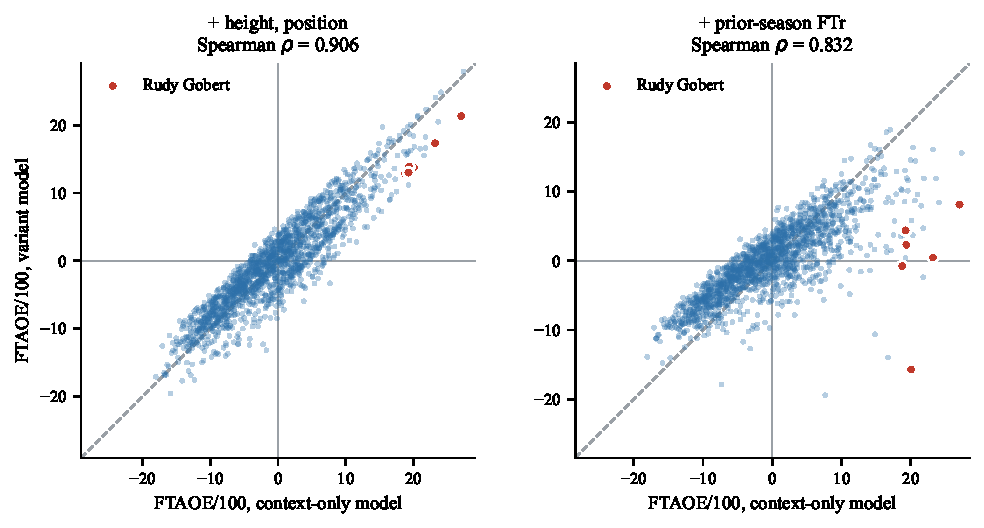
\includegraphics[width=\textwidth]{figures/fig3_identity_variant.pdf}
\caption{FTAOE per 100 under the context-only model against two identity-aware
variants. Gobert's six seasons highlighted.}
\label{fig:identity}
\end{figure}

\subsection{Who it finds}

The 2024--25 leaders are Giannis Antetokounmpo ($+311.8$), James Harden
($+192.5$), Jimmy Butler III ($+190.7$) and Shai Gilgeous-Alexander ($+175.0$);
the bottom is Mikal Bridges ($-120.0$), Klay Thompson ($-104.5$), Payton
Pritchard ($-103.7$) and Buddy Hield ($-97.3$). The list is unsurprising, which
is the check: a metric that put unfamiliar names on top would be measuring noise,
and this one recovers the recognised foul-drawers without ever being told who
they are.

It also separates players a single efficiency number merges. Across seasons
Stephen Curry is $+5.4$ percentage points on shot-making with FTAOE of $-23$:
elite shot-maker, below-expectation foul-drawer. That is two different skills,
and folding them into one number hides it.

\section{What a team can do with this}

\textbf{Use it in-season, with a known error bar.} Because $K = 67$, a player
passes $r = 0.5$ at about 67 finisher-possessions and $r = 0.9$ at about 600.
That is roughly two months of a rotation player's usage, so FTAOE is usable well
before the season ends. It also stabilises considerably faster than most
box-score rate statistics. The flip side is a hard limit: separating two players
20 possessions apart is not something this metric supports, and the padding
constant tells you so explicitly rather than leaving you to guess.

\textbf{Evaluate the skill, not the role.} In scouting and contract work, raw
free-throw attempts systematically flatter high-usage rim finishers and penalise
off-ball shooters. FTAOE prices the residual. Curry above is the clean
illustration: a team paying for foul-drawing on raw FTA would misread him in both
directions depending on the season's usage.

\textbf{Compare across seasons and rule changes.} Season anchoring means a
league-wide enforcement shift, like the 2021--22 crackdown on non-basketball
shooting motions, does not leak into every player's number as a common offset.
Multi-year projection off unanchored FTA per game will absorb that shift as if it
were player change.

\textbf{Separate officiating from the player.} The crew term is positive in every
fold (1.71 to 2.53 on a rate scale where the league mean is 0.18). Crews differ
enough to move a player's expected free-throw total over a season, so a team can
quantify how much of a player's swing is schedule and assignment rather than
form. We stop short of any bias claim: crew assignment is not random with respect
to teams, venues or scheduling, and this design cannot support one.

\textbf{Extending it.} The same construction needs only public play-by-play with
foul attribution, and we have run the pipeline on eight non-NBA leagues, though
the reliability analysis here is NBA-only.

\section{Limitations}

FTAOE measures foul-drawing given the possessions a player finished, so skill at
\emph{choosing} contact-prone situations sits inside the residual rather than the
baseline; separating contact craft from shot selection needs a selection model we
have not built \citep{sandholtz2020measuring}. Without tracking data there is no
defender distance, shot clock or touch time, which caps the companion shot model
near AUC 0.66 and removes the most plausible physical mediator of foul drawing.
Calibration is unbiased in aggregate (\SI{0.95}{\percent}) but weak across the
model's own predicted deciles (slope 0.426), which is expected for a context-only
model and means these predictions should not be used to rank player-season rates
directly. The leakage comparison rests on a single held-out season, 2024--25.

\vspace{1mm}
\noindent\footnotesize
\textbf{Reproducibility.} Code, model artifacts and the scripts producing every
figure are in the repository on the title page. The two variant comparisons each
assert that their baseline arm reproduces the shipped model before their variant
arms are read. This paper is condensed from a longer manuscript; all numbers are
drawn from the same claims ledger.

\bibliography{references}

\end{document}
